% Dokument:
\documentclass[a4paper,10pt,onecolumn]{article}
\usepackage[utf8]{inputenc}
%\usepackage[norsk]{babel}
\usepackage{hyperref}

% Formatering:
\usepackage{geometry,amsthm,blindtext}
\setlength{\parindent}{0mm}
\setlength{\parskip}{1.8mm}
% Symboler
\usepackage[geometry]{ifsym}
% Matematikk:
\usepackage{amsmath,mathtools,amsfonts,xparse,physics,esint,mathrsfs,nicefrac,siunitx}
% Kode:
\usepackage{verbatim,listings,algpseudocode}
% Tekst:
\usepackage{textcomp,varioref,enumerate,bbold}
% Figurer:
\usepackage{graphicx,subcaption,float,dcolumn,multirow}
\usepackage[section]{placeins}
% Farge:
\usepackage{xcolor}

% Dcolumn-kolonner
\newcolumntype{,}{D{,}{{,}}{2}}
\newcolumntype{=}{D{=}{=}{-1}}
\newcolumntype{.}{D{.}{{.}}{2}}
\newcolumntype{C}{>{$}c<{$}}

% Listings-Instillinger
	\lstset{
	% Språk
	language=c++,
	% Farge
	backgroundcolor=	\color[rgb]{0.9,0.9,0.9},
	keywordstyle=		\color[rgb]{0,0,1},
        	commentstyle=		\color[rgb]{0.133,0.545,0.133},
        	stringstyle=		\color[rgb]{0.627,0.126,0.941},
	numberstyle=\tiny	\color[rgb]{0.5,0.5,0.5},
        	rulecolor=			\color{black},
	% Tekst:
	basicstyle=\scriptsize,
	showspaces=false,
	showstringspaces=false,
	showtabs=false,
	% Spesialtegn
	extendedchars=true,
        	literate=	{æ}{{\ae}}1 	{ø}{{\o}}1 		{å}{{\r a}}1 
		  	{≤}{{$\leq$}}1 	{≥}{{$\geq}}1	{–}{{$-$}}1		{~}{{\tiny{$\sim$}}}1,
        	% Format
	frame=single,
	aboveskip={1.5\baselineskip},
	breaklines=true,
	columns=fixed,
	numbers=left,
	numbersep=5pt,
	stepnumber=1,
	tabsize=4, 
	% ... 
        	upquote=true,
        	prebreak = \raisebox{0ex}[0ex][0ex]{\ensuremath{\hookleftarrow}},
        	identifierstyle=\ttfamily
        	}
	
% Nummerering:
%\renewcommand{\thesection}{\arabic{section}}		% Nummer i "section"
%\renewcommand{\thessubection}\arabic{subsection}}	% Nummer i "subsection"
%\renewcommand{\thesection}{\alph{section}}			% Bokstaver i ''section''
%\renewcommand{\thesubsection}{\alph{subsection}}	% Bokstaver i ''subsection''

% Egendefinerte kommandoer:
	% Snarveier
	\newcommand*{\eqset}[1]{\begin{dcases}#1\end{dcases}}
	\newcommand*{\Qfig}[3]{\begin{figure}[ht]	\centering \includegraphics[#2]{#1} \caption{#3} \end{figure} }
	% Tegn
	\newcommand{\point}{\varointclockwise}	% integral med klokken
	\newcommand{\noint}{\ointctrclockwise}	% integral mot klokken
	\newcommand{\ee}[1]{\!\times\!\!10^{#1}} 	% 10 i #1-te
	\newcommand{\un}[1]{\,\si{#1}}		% enheter
	\newcommand{\e}[1]{\mathrm{e}^{#1}}	% exp()
	\newcommand{\ci}{\dot{\iota\!\:}}		% kompleks i
	% misc
	\newcommand{\note}[1]{{\color{red}\quad[$\backslash!/$: #1]}}	% notater for dokument under arbeid
	\newlength{\txtsz}\makeatletter\setlength{\txtsz}{\f@size pt}\makeatother
	\newcommand{\insubsec}[1]{\par{\bf #1}}

% Åpning:
\title{Studies of phase transitions in magnetic systems}
\author{Johannes Sørby Heines}


% START
\begin{document}

%\twocolumn[
%\begin{@twocolumnfalse}
\maketitle
\begin{abstract}
We implement the Metropolis algorithm in order to simulate the two dimensional Ising model. The program is tested agains theoretical calculations for a $2\times2$ lattice, and its dependence on the number of Monte Carlo cycles is studied. The program is subsequently applied to lattices up to $100\times100$ in order to study the phase transitions. 
\end{abstract}
%\end{@twocolumnfalse}
%]

\section{Introduction}

A phase transition is a sudden change in the physical properties of a system. In the case of a spin lattice, this property is the magnetization. At low temperatures, it's energetically favourable for the spins to be aligned, giving rise to a spontaneous magnetization $\expval{M}\neq0$. For high temperatures, however, the spins are randomized, giving no mean magnetization: $\expval{M} = 0$. The temperature at which this change occurs is called the critical temperature, denoted $T_C$.

We give a brief overview of the Ising model and its modeling of phase transitions, outline the Metropolis algorithm, and apply it to multiple two dimensional lattices.
We study the behaviour of the algorithm as functions of Monte Carlo cycles, and of the system as functions of temperature.
We finally use our simulations of heat capacity $C_V$ and susceptibility  $\chi$ to estimate the critical temperature $T_C$ for an infinitely large lattice.  

%
%
%
\section{Theoretical models and implementation}

\subsection{The Ising model}\label{sec:ising}

The Ising model is a simple model of magnetic systems, where each spin only interacts with its neighbours. The resulting energy of the system, when placed in an external magnetic field $\mathcal{B}$, is given by
\begin{equation}\label{eq:ising}
E = -J \sum_{<kl>}^Ns_ks_l - \mathcal{B}\sum_{k}^Ns_k,
\end{equation}
where $J$ is a coupling constant, $N$ is the total number of spins, $s_k = \pm1$ represents one spin and the notation $<kl>$ indicates summation over the immediate neighbours only. 

In this project, we will study a two dimensional spin lattice with no external magnetic field.  

Since the energy depends on the coupling of neighbouring spins, we must define boundary conditions when working with a finite lattice. We will use periodic boundary conditions, where each edge of the lattice is used as the boundary for the opposite edge. 

For a $2\times2$ lattice with periodic boundary conditions, the Ising model has a simple analytic solution. 
This case has $2^4=16$ microstates, but only six macrostates, listed in table \ref{tab:2x2}. 

\begin{table}
	\centering
	\caption{The possible macrostates for a $2\times2$ spin lattice with periodic boundary conditions}
	\label{tab:2x2}
	\begin{tabular}{|l|l|>{$}r<{$}|r|}\hline
	Number of spins up & Degeneracy & \text{Energy} & Magnetization\\\hline
	4 & 1 & -8J & 4	\\
	3 & 4 & 0 & 2	\\
	2 & 4 & 0 & 0 	\\
	2 & 2 & 8J & 0	\\
	1 & 4 & 0 & -2	\\
	0 & 1 & -8J & -4 \\\hline
	\end{tabular}
\end{table} 
One microstate for each of the first four macrostates is shown below:
\[
\mqty{\uparrow&\uparrow\\\uparrow&\uparrow} \qq{;}
\mqty{\uparrow&\uparrow\\\uparrow&\downarrow} \qq{;}
\mqty{\uparrow&\downarrow\\\downarrow&\uparrow} \qq{;}
\mqty{\uparrow&\uparrow\\\downarrow&\downarrow} \qq{.}
\]


%the energy of a microstate $i$ is given as
%\[
%E_i = -J(s_1s_2+s_2s_1+s_1s_3+s_3s_1+s_2s_4+s_4s_2+s_3s_4+s_4s_3).
%\] 
%\note{reproduce and explain table}
%If all spins are aligned, then $E_i=-8J$. If $s_1=s_4=-s_2=-s_3$, then $E_i=8J$. For all other configurations, $E_i=0$. 

We can calculate the partition function 
\[
Z = \sum_i\e{-E_i\beta} = 2\e{8J\beta} + 2\e{-8J\beta} + 12\e{0} = 4\cosh(8J\beta) + 12,
\]
where $\beta = 1/k_BT$. This allows us to find analytical expressions for the expectation values in the $2\times2$ case. 
We can scale the expressions by using 
$T^* = Tk_B/J = 1/J\beta$, 
$E^* = E/J$,
$C_V^* = C_V/k_B$ and
$\chi^* = J\chi$.
Throughout this report, in order to avoid clutter, we will drop the $^*$ and always use the scaled variables unless stated otherwise.
We then get the following expectation values.

Energy:
\begin{align*}
\expval{E} = \frac{1}{Z}\sum E_i\e{-E_i/T} = \frac{2\cdot8\e{-8/T}+2\cdot(-8)\e{8/T}}{4\cosh(8/T)+12}
\qcomma \expval{E^2} = \frac{2\cdot8^2\e{-8/T}+2\cdot(-8)^2\e{8/T}}{4\cosh(8/T)+12}
\end{align*}
Magnetization: 
\[
\expval{\abs{M}} = \frac{1}{Z}\sum \abs{M_i}\e{-\beta E_i} = \frac{2\cdot4\e{8/T} + 8\cdot2}{4\cosh(8/T)+12}
\qcomma
\expval{M^2} = \frac{2\cdot4^2\e{8/T} + 8\cdot2^2}{4\cosh(8/T) + 12}
\]
Heat capacity:
\begin{align*}
\expval{C_V} &= \frac{\expval{E^2}-\expval{E}^2}{T^2} 
%= \frac{1}{T^2}\qty[\frac{16^2\e{-8/T}-16^2\e{8/T}}{4\cosh(8/T)+12} - \qty(\frac{16\e{-8/T}-16\e{8/T}}{4\cosh(8/T)+12})^2]
%\\&= \frac{1}{T^2}\qty[\frac{16^2\e{-8/T} - 16^2\e{8/T}}{4\cosh(8/T)+12} - \frac{16^2\e{-8/T}+16^2\e{8/T} - 32}{16\cosh[2](8/T) + 96\cosh(8/T) + 144}]
%\\&= \frac{1}{T^2}\qty[\frac{64\e{-8/T} - 64\e{8/T}}{\cosh(8/T)+3} - \frac{16\e{-8/T}+16\e{8/T} - 32}{\cosh[2](8/T) + 6\cosh(8/T) + 9}]
\end{align*}
Magnetic susceptibility:
\[
\expval{\chi} = \frac{\expval{M^2} - \expval{\abs{M}}^2}{T}  
\]

These analytic expressions were used as benchmark calculations for the algorithm. 

\subsection{Phase transitions}
The two dimensional Ising model undergoes a second order phase transition. In the thermodynamic limit $L\to\infty$, the magnetization goes to zero with an infinite slope at the critical temperature. 
The heat capacity and magnetic susceptibility  both diverge. \cite{lecture}

For a finite lattice, we will not observe any divergence, but a sharp peak in both heat capacity and susceptibility close to the critical temperature. Similarly, the magnetization will not have an infinite slope towards zero, but rather a steep decrease followed by a tail \cite{lecture}.

The critical temperature for a finite lattice of side length $L$ can be related to the critical temperature in the thermodynamic limit by the expression \cite{lecture}
\begin{equation}\label{eq:Tc}
T_C(L) - T_C(L=\infty) = aL^{-1/\nu},
\end{equation}
where $a$ is a constant and $\nu=1$ is a known critical exponent. 

The critical temperature for an infinite lattice was calculated analytically by Lars Onsager and is \cite{labtext}
\begin{equation}\label{eq:exact}
T_C(L=\infty) = \frac{2}{\ln(1+\sqrt{2})} \approx 2.269. 
\end{equation}

\subsection{The Metropolis algorithm}
%We simulated the system using the Metropolis algorithm. This algorithm is based on Monte Carlo 
The Metropolis algorithm a method of sampling the possible distributions of a system. As the number of samples becomes very large, we expect the sample distribution to approach the actual distribution. 
In our case, we are interested in the spin distribution of the two-dimensional square lattice at a given temperature.   
 
For two states $i$ and $j$ of the system, the Metropolis algorithm accepts the transition $j\to i$ if 
\[
r \leq \frac{w_i}{w_j} = w = \e{-\Delta E/T},
\]
where $r$ is a random number in $[0,1]$ from a uniform probability distribution function (pdf), and $\Delta E = E_i-E_j$ is the energy difference between the two states \cite{lecture}. 

When running our algorithm, we can chose to make transitions by flipping one random spin in the lattice. Each spin $s_l$ interacts equally with its four neighbours $s_k$, giving it five possible energies depending on the number of neighbours aligned to it, from none to all four. 
Thus, flipping a single spin can only result in one of five different values for $\Delta E$, given by
\begin{equation}
\Delta E = 2s_l\sum_{<k>}^Ns_k = \{-8,-4,0,4,8\}.
\end{equation} 
This means that the expression $\exp(-\Delta E/T)$ can be precalculated for each $\Delta E$. For each transition the algorithm only calculates $\Delta E$, and simply looks up the corresponding $w$.      

One Monte Carlo cycle for the Metropolis algorithm can be expressed as follows
\begin{algorithmic}
\For{$i = [0:1:L^2]$}
\State Pick a random spin $s_l$ form the lattice $S$
\State $\Delta E := 2s_l\sum_{<k>}^N s_k$
\State $\Delta M := -2s_l$
\State Pick a random number $r \in [0,1]$ from a uniform pdf
\If{$r \leq w$}
\State $s_l := -s_l$
\State $E := E+\Delta E$
\State $M := M+\Delta M$
\EndIf
\EndFor
\end{algorithmic}

Another issue when implementing this algorithm is the encoding of periodic boundary conditions. Testing wether the proposed transition is at a boundary will slow the program down considerably \cite{optimize}.  
We have chosen to add the boundaries directly to the spin matrix in the following way:
\[
\bmqty{
 & s_{1L} & \cdots & s_{LL} & \\
s_{L1} & s_{11}&\cdots&s_{L1} & s_{11}\\
\vdots & \vdots&&\vdots& \vdots\\
s_{LL} & s_{1L}&\cdots&s_{LL} & s_{1L}\\
 & s_{11} & \cdots & s_{L1} & }
\]
To avoiding If-tests we update all boundaries at every iteration. This adds $4L$ writes per iteration, but no FLOPs. 
Another possibility would be to use circular indexing, which can be implemented by the expression \((i\mod L + L)\mod L\). This adds 3 FLOPs per iteration. 


\section{Methods}

We studied the behaviour of the Metropolis algorithm as a function of the number of Monte Carlo cycles for a $20\times20$ spin lattice. We ran the simulation for the temperatures of 1.0 and 2.4 in our scaled units, and in each case for both aligned and randomized spins at the start. 

We also estimated the probability $P(E)$ of the $20\times20$ lattice being in a state with energy $E$ for the same two temperatures. This was done by counting the number of times a given energy appeared in the calculations after the steady state had been reached. For these simulations, we started with aligned spins for $T=1.0$ and randomized spins for $T=2.4$. 

In order to study the phase transitions of the Ising model, we performed simulations for lattices with $L\in\{40,60,80,100\}$.

The temperatures corresponding to the top of the peaks in $\chi(T)$ were used to fit equation \ref{eq:Tc} with $a$ and $T_C(L=\infty)$ as fitting parameters.
This fit was also performed for the temperatures corresponding to the peaks in $C_V(T)$. 

%
%
%
\section{Results}

\subsection{The $2\times2$ lattice}
Figure \ref{fig:2x2} shows the results of a simulation with one million Monte Carlo cycles for a $2\times2$ lattice, along with the theoretical expectation values calculated in section \ref{sec:ising}. The error in the simulated values is plotted in figure \ref{fig:2x2err}.

\begin{figure}
	\centering
	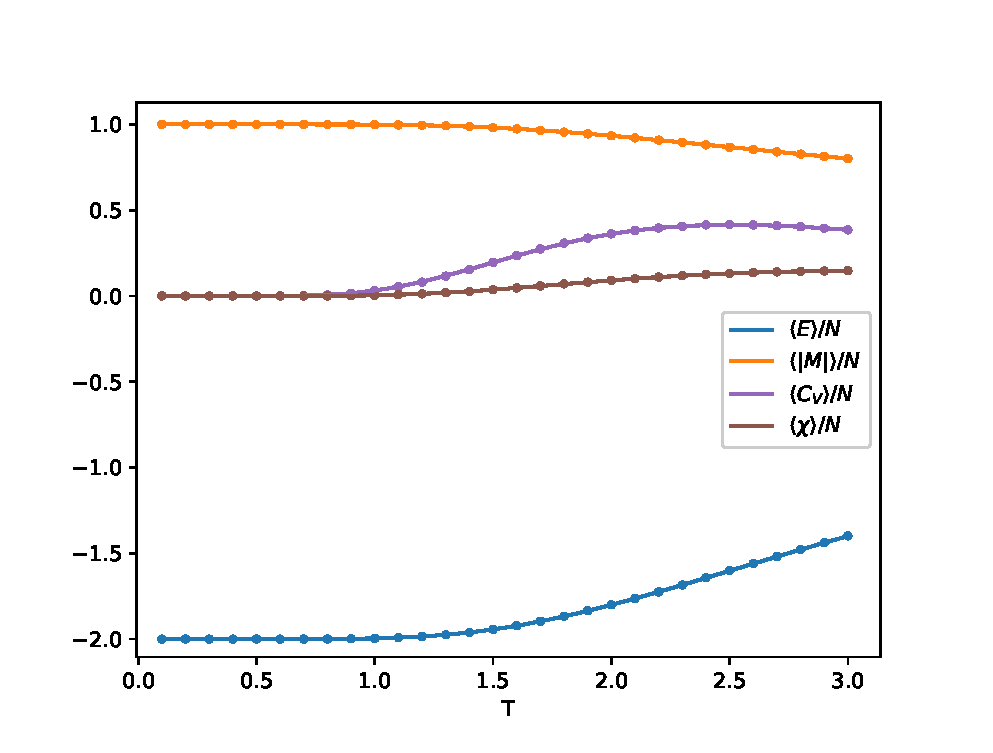
\includegraphics[width=\linewidth]{2x2.eps}
	\caption{The expectation values for a $2\times2$ lattice as functions of temperature. The points were calculated with the Metropolis algorithm over 1\,000\,000 Monte Carlo cycles, discarding the first 10\,000. The lines show the theoretical functions given in section \ref{sec:ising}.}
	\label{fig:2x2}
\end{figure}

\begin{figure}
	\centering
	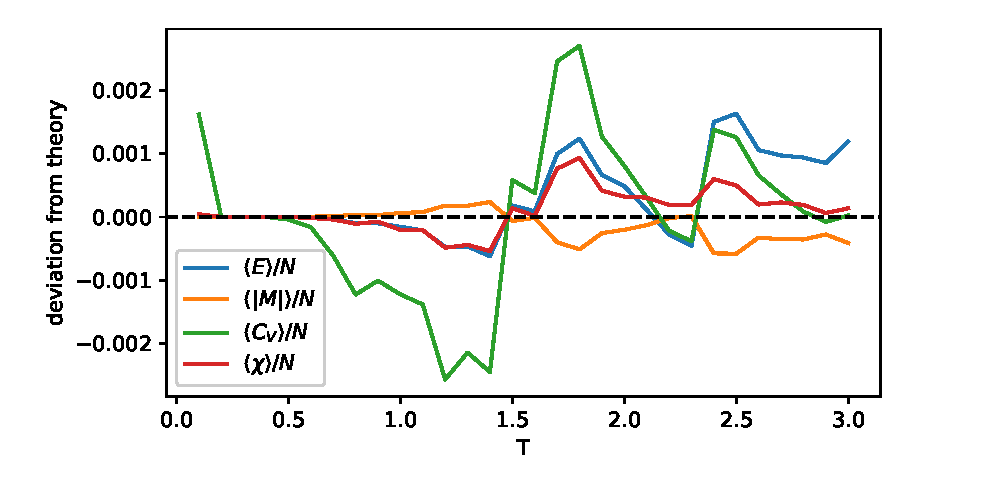
\includegraphics[width=\linewidth]{2x2err.eps}
	\caption{The difference between the simulated and analytical values plotted in figure \ref{fig:2x2}.}
	\label{fig:2x2err}
\end{figure}

\subsection{Equilibration time}
Figure \ref{fig:eq} shows the expectation values of energy and magnetization, as well as the number of accepted configurations, as functions of the number of Monte Carlo cycles. The values come from a simulation with a $20\times20$ spin lattice.

\begin{figure}
	\centering
	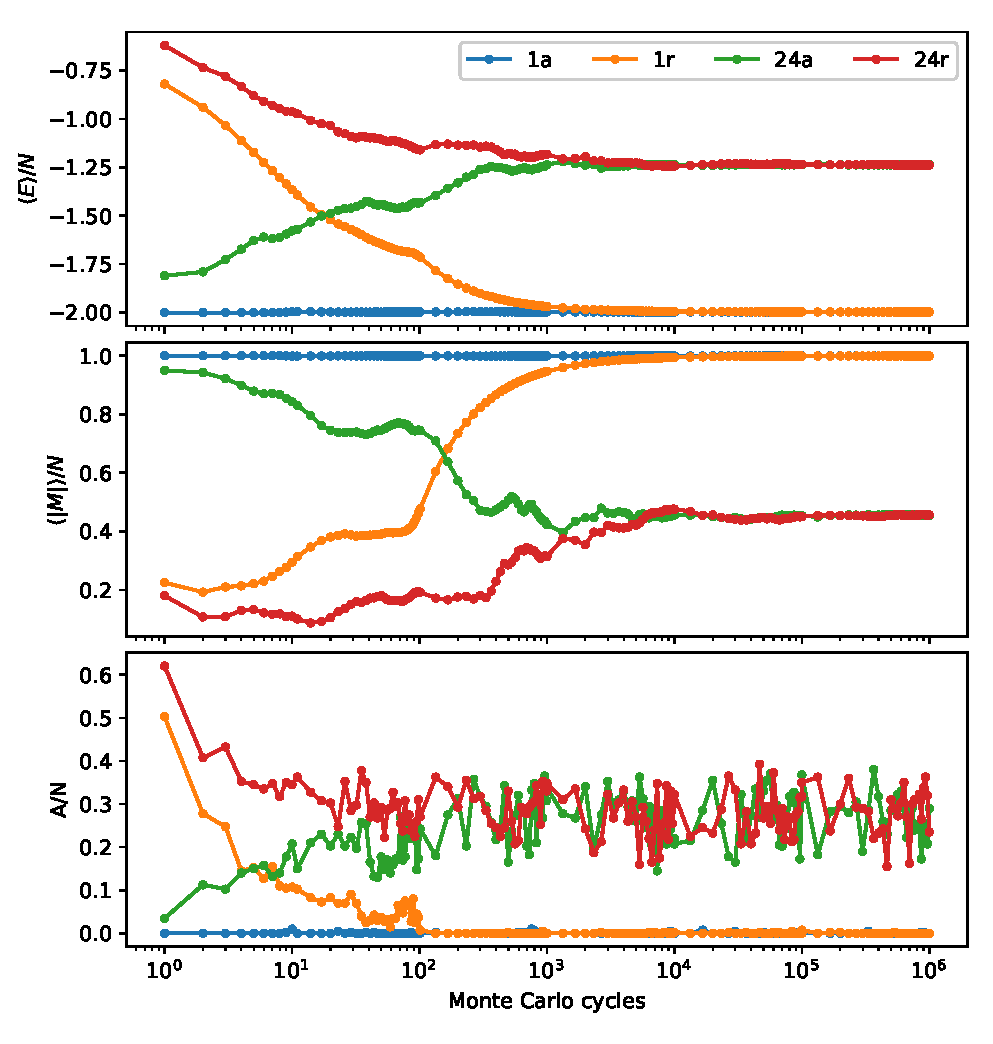
\includegraphics[width=\linewidth]{20mcs.eps}
	\caption{Mean energy $\expval{E}$, mean absolute magnetization $\expval{\abs{M}}$ and number of accepted configurations $A$, per spin, for a $20\times20$ lattice. The simulations were done for $T=\{1.0,2.4\}$ (1 and 24 in the legend) and with spins initially aligned or randomized (a and r in the legend).}
	\label{fig:eq}
\end{figure}

\subsection{Energy probability distribution}
Figure \ref{fig:hist} shows the energy distribution after the $10\,000^\mathrm{th}$ Monte Carlo cycle for the same $20\times20$ lattice as above. 

\begin{figure}
	\centering
	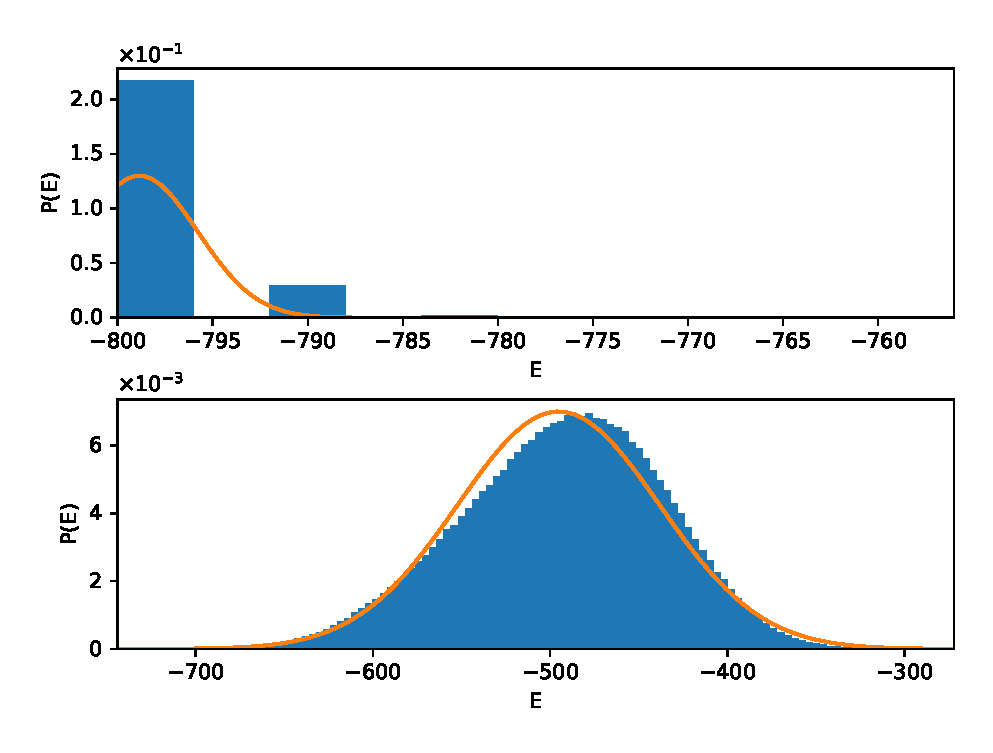
\includegraphics[width=\linewidth]{hist.eps}
	\caption{Histogram approximating the probability $P(E)$ of a $20\times20$ lattice for temperatures $T=1.0$ (top) and $T=2.4$ (bottom). The curves shows a normal distribution with the mean and standard deviation of the energy values.}
	\label{fig:hist}
\end{figure}

\subsection{Phase transitions and critical temperature}	
Figures \ref{fig:exp} show the studied expectation values as functions of temperature for lattices with side length $L=\{20,60,80,100\}$. 
The tops of the peaks in heat capacity were found by a Gaussian fit, also shown in figure \ref{fig:C}. The tops in susceptibility (figure \ref{fig:X}) were determined by eye, this will be discussed later.

\begin{figure}
	\centering
	\begin{subfigure}{0.5\linewidth}
		\centering
		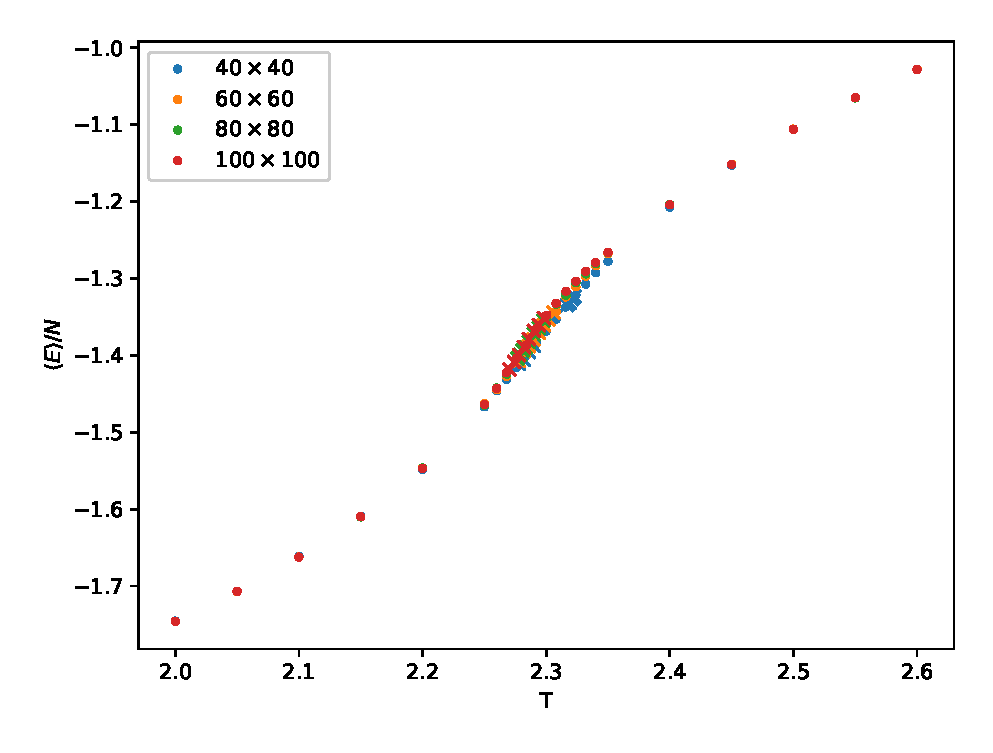
\includegraphics[width=\linewidth]{energy.eps}
		\caption{Energy per spin}
		\label{fig:E}
	\end{subfigure}%
	\begin{subfigure}{0.5\linewidth}
		\centering
		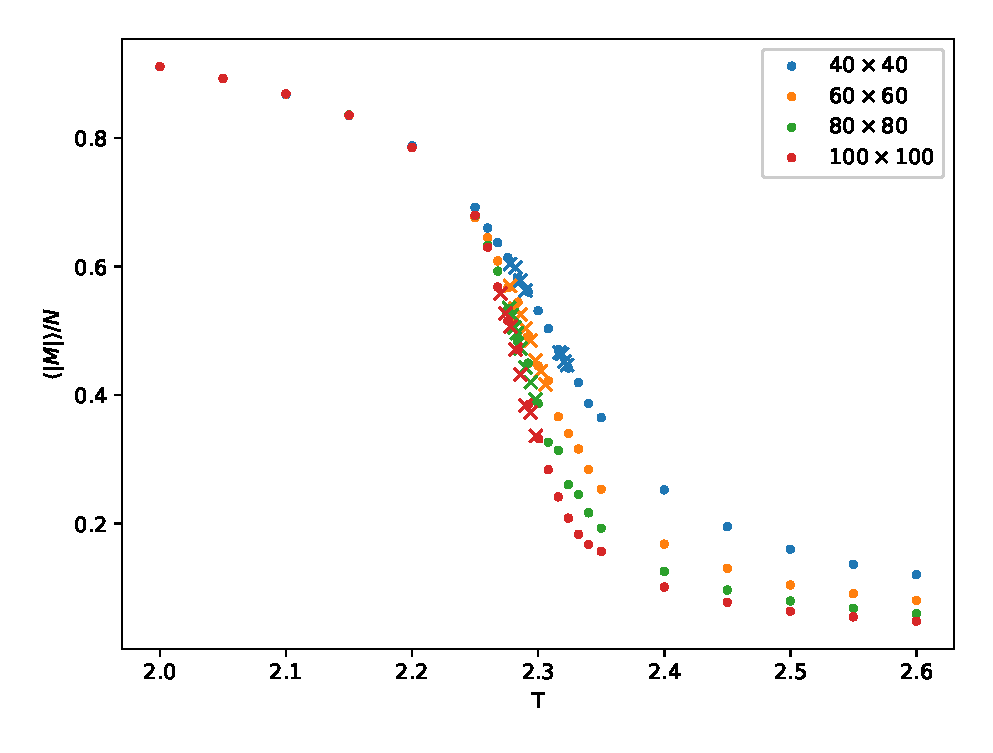
\includegraphics[width=\linewidth]{magnetization.eps}
		\caption{Absolute magnetization per spin}
		\label{fig:M}
	\end{subfigure}
	\begin{subfigure}{0.5\linewidth}
		\centering
		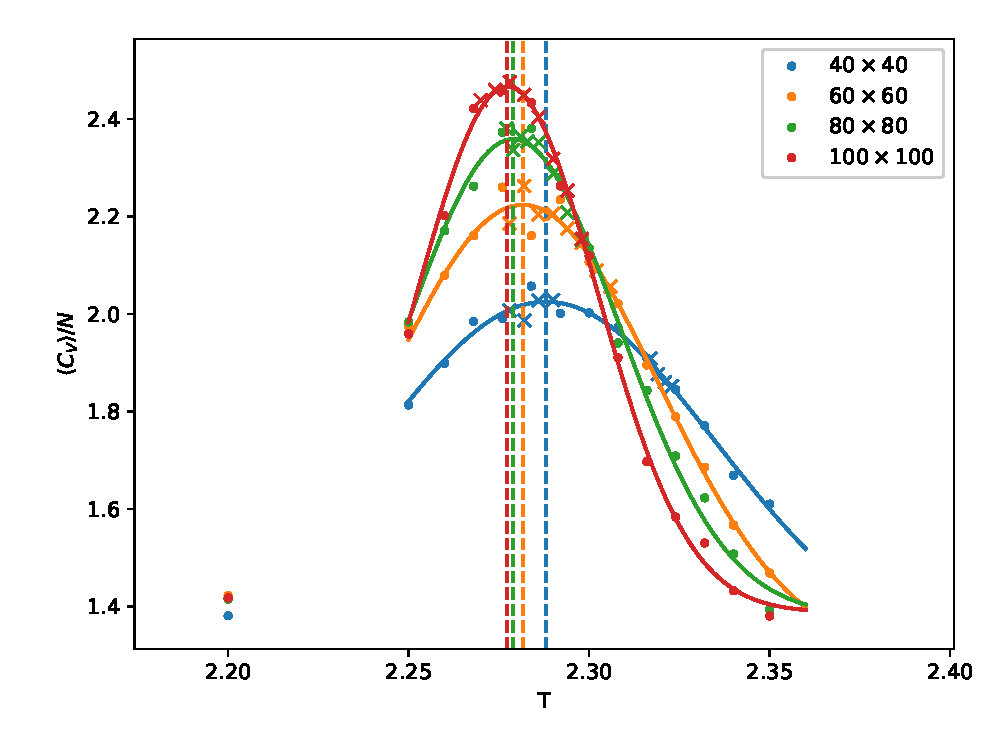
\includegraphics[width=\linewidth]{heatcapacity.eps}
		\caption{Heat capacity per spin}
		\label{fig:C}
	\end{subfigure}%
	\begin{subfigure}{0.5\linewidth}
		\centering
		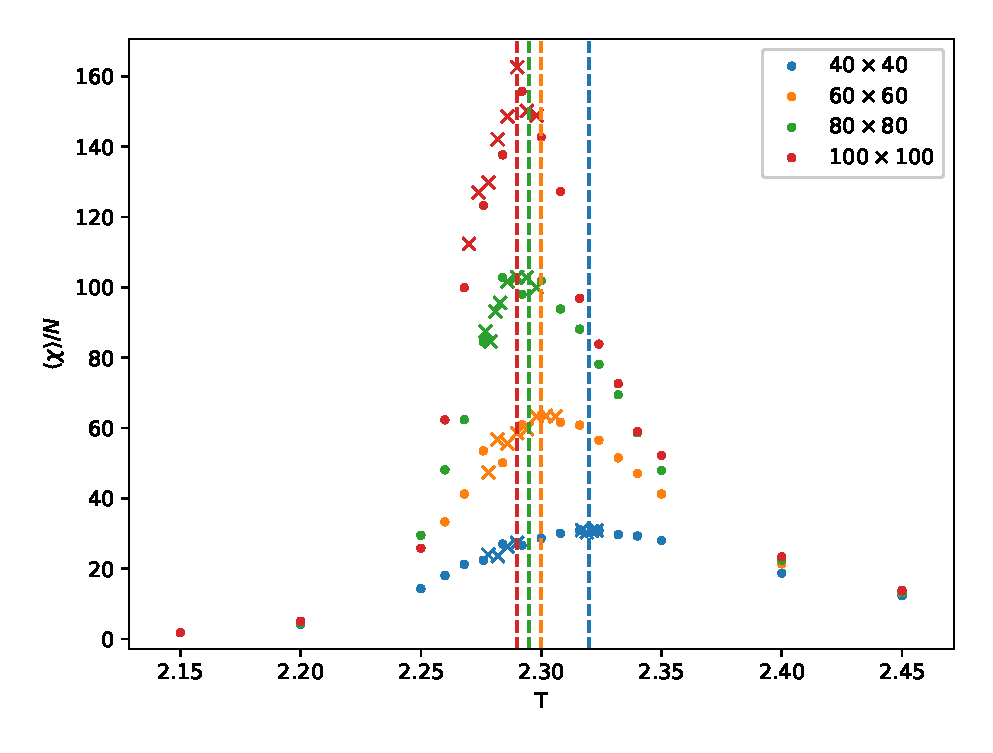
\includegraphics[width=\linewidth]{susceptibility.eps}
		\caption{Susceptibility per spin}
		\label{fig:X}
	\end{subfigure}
	\caption{Expectation values as functions of temperature for different lattice sizes. The values marked by dots were found with $10^6$ Monte Carlo cycles, while those marked with $\cross$ were found this $3\ee{6}$ cycles. The dashed lines mark estimated maxima. These were determined from a Gaussian fit for the heat capacity $C_V$ and by eye for the susceptibility $\chi$.}
	\label{fig:exp}
\end{figure}

A fit of the critical temperatures estimated from the susceptibility to equation \ref{eq:Tc} yields 
\[T_C(L=\infty) = 2.2694 \qand a = 1.9839.\] 
A fit to the same equation of the critical temperatures estimated from the heat capacity yields 
\[T_C(L=\infty) = 2.26997 \qand a = 0.71755.\] 
 

%
%
%
\section{Discussion}
Our comparison with the known analytical solution for the $2\times2$ matrix shows a good agreement, with a relative error of the order of $0.1\%$ for both energy and magnetization (figures \ref{fig:2x2} and \ref{fig:2x2err}). This mainly serves to justify the further use of the program for the other experiments.

For a temperature of $T=1.0$, much lower than the critical temperature, we expect most of the spins to be aligned. This is consistent with what we observe in figure \ref{fig:eq} for energy and magnetization. 
The temperature of $T=2.4$ is high enough that spins start to flip, decreasing the total magnetization and increasing the energy. 
In both cases, the steady state is reached after approximately 10\,000 Monte Carlo cycles. However, in the case where the spins start out aligned at $T=1.0$, the steady state is reach almost immediately. 
This illustrates that having  a good approximation of the steady state is very advantageous when performing this type of simulation.

The number of accepted configurations is close to zero for $T=1.0$. For $T=2.4$ it is both higher and much more unstable, varying between approximately 0.15 and 0.35 accepted configurations per spin.
This is directly related to the entropy of the two macrostates: There are many more microstates with $T=2.4$ than there are with $T=1.0$ after equilibration, thus more configurations are accepted, and more variation is possible. 

As expected, the probability distributions in figure \ref{fig:hist} show a narrow peak for $T=1.0$ and a much wider peak at $T=2.4$. We notice in the latter case, though it might also be the case in the former, that the distribution is not Gaussian, but is skewed towards zero.
%According to the central limit theorem \cite{lecture} the means of multiple independent samples from any\footnote{Under certain conditions which we will not discuss here. The distributions for which it does not apply are very rarely encountered in physics.} distribution are normally distributed. 
%Discarding more Monte Carlo cycles does not have any effect on this 
%This suggests that our measurements are not perfectly independent, which is reasonable considering that the state of the system at one point determines which states are possible at the next point. We have not however been able to verify wether this is enough to account for the observed skewness.

The behaviour of the expectation values in figure \ref{fig:exp} shows clear evidence of phase transitions. We observe the sudden decrease in magnetization around the critical temperature – not to zero as we study finite lattices – and the expected peaks in heat capacity and susceptibility. 
The peaks of heat capacity gave seemingly reasonable fits to a Gaussian plus a constant, but this proved impossible for the peaks in susceptibility. 
As we were unable to find a working fit function, we chose to determine the top by eye. For the $60\times60$ and $100\times100$ case, this simply meant choosing the highest point. 
For the others, the highest data point was visibly displaced when compared to the surrounding points. We then placed the maximum based on the overall shape of the data around that point.
 
A future study should run the calculations with more cycles around these points, and determine a suitable fitting function.

Despite the important error sources described above, the estimates for the critical temperature in the thermodynamical limit are in good agreement with the theoretical value \ref{eq:exact}. We got the value $T_C = 2.2694$ from the susceptibility, and $T_C = 2.26997$ from the  heat capacity. The relative errors of these values are 0.014\% and 0.045\% , respectively.    


%
%
%
\section{Conclusion}
We implemented the metropolis algorithm for solving the two dimensional Ising model. 

Our program's calculations were in good agreement with theory for the $2\times2$ case, and reproduced well the expected behaviour of the expectation values. 

The computed $P(E)$ distribution also behaved as expected, but was slightly skewed towards zero. 

We finally used our simulations of heat capacity and susceptibility to calculate estimates of the critical temperature at the thermodynamic limit. Our values were consistent with the theoretical $kT_C/J = 2/\ln(1+\sqrt{2}) \approx 2.269$ to within 0.014\% and 0.045\% respectively. 


%\onecolumn
\begin{thebibliography}{9}

\bibitem{labtext}
Morten Hjorth-Jensen. Project 4. 2020. \textsc{url: }\url{http://compphysics.github.io/ComputationalPhysics/doc/Projects/2020/Project4/html/Project4.html}

\bibitem{lecture}
Morten Hjorth-Jensen. Computational Physics Lectures. 2015. \textsc{url: }\url{https://github.com/johashei/ComputationalPhysics/blob/master/doc/Lectures/lectures2015.pdf}

\bibitem{optimize}
Morten Hjorth-Jensen. Computational Physics Lectures: How to optimize codes, from vectorization to parallelization. 2020. \textsc{url: }\url{http://compphysics.github.io/ComputationalPhysics/doc/pub/codeoptimization/html/codeoptimization.html}


\end{thebibliography}



% Husk å avslutte alle environments
% SLUTT
\end{document}